%%%%%%%%%%%%%%%%%%%%%%%%%% lecture-17
%\begin{frame}[shrink]
%\frametitle{lecture-17 主要内容}
%\framesubtitle{结构体编程举例续}
%%\tableofcontents[hideallsubsections]
%\tableofcontents
%\medskip
%\textbf{\textcolor{blue}{训练编程逻辑思维方式:}}
%\begin{itemize}
%	\item 领会结构化(模块化)编程思想。 
%	\item 用结构体管理相互关联的数据, 使其成为结构化的整体数据, 便于统一处理。 
%	\item 大问题分解为小问题, 设计函数解决小问题, 各个子函数彼此之间相互独立(便于调试, 不易出错),又可通过参数和返回值传递数据。
%	\item 主程序调用各个子函数, 解决``大"问题。
%\end{itemize}
%\end{frame}

\begin{frame}[shrink,fragile]{例6: 复试赛选}
\begin{tikzpicture}
\node[text width=.7\textwidth] (t) {
	考研初试成绩公布后需要对$m$个学生的成绩进行排序,筛选出可以进入复试的前n名学生。
	排序规则为首先按照总分排序,总分相同则按英语单科成绩排序,总分和英语成绩也相同时考号小者排在前面。
	
	现给出这$m$个学生的考研初试成绩,请筛选出可以进入复试的n名学生并按照排名从高到低的顺序依次输出。
	
	\textcolor{blue}{输入说明:} 输入为$m+1$行,第一行为两个整数$m$和$n$,分别表示总人数和可以进入复试人数,$m$和$n$之间用空格分隔,$0<n<m<200$。接下来为$m$行数据,每行包括三项信息,分别表示一个学生的考号(长度不超过20的字符串)、总成绩(小于500的整数)和英语单科成绩(小于100的整数),这三项之间用空格分隔。
	
	\textcolor{blue}{输出说明:} 按排名从高到低的顺序输出进入复试的这n名学生的信息。
};
\node[anchor=west,text width=.3\textwidth,draw] at($(t.east)+(0.5,0)$) {
输入样例\\	
5 3\\
XD20160001 330 65\\
XD20160002 330 70\\
XD20160003 340 60\\
XD20160004 310 80\\
XD20160005 360 75

输出样例\\	
XD20160005 360 75\\
XD20160003 340 60\\
XD20160002 330 70
};
\end{tikzpicture}
\end{frame}

\begin{frame}[shrink,fragile]{例6: 复试赛选, 定义结构体}
\begin{columns}[T]
\column{0.5\textwidth}
\textbf{\textcolor{blue}{思路:}}
\begin{enumerate}
	\item 定义考生结构体, 各考生组成结构体数组;
	\item 按要求对结构体数组进行排序。
\end{enumerate}
\column{0.4\textwidth}
\begin{lstlisting}
#include<stdio.h>
// 字符串比较函数strcmp(s1,s2);
#include<string.h> 
#define N 200 // 估计的考生数
// 定义结构体
struct Student 
{ 
   char no[20]; // 考号
   int  total;  // 总成绩
   int  english;// 英语成绩
};
\end{lstlisting}
\end{columns}
\end{frame}

\begin{frame}[shrink,fragile]{例6: 复试赛选(结构体数组), 输入输出}
\vspace{-0.4cm}
\begin{lstlisting}
// 输入m个考生信息
void input(struct Student *stus, int m) 
{
  int i;
  for(i=0;i<m;i++) 
    scanf("%s%d%d",stus[i].no,&stus[i].total,&stus[i].english); 
}
// 输出n个考生信息
void print(struct Student *stus, int n) 
{
  int i;
  for(i=0;i<n;i++) 
    printf("%s %d %d\n",stus[i].no,stus[i].total,stus[i].english); 
}
\end{lstlisting}
\end{frame}

\begin{frame}[shrink,fragile]{例6: 复试赛选(结构体数组),交换函数}
\begin{columns}[T]
\column{0.8\textwidth}
\begin{lstlisting}
// 交换两个结构体指针的内容, 地址传递
// 两个结构体的各数据成员互相交换 
void swap(struct Student *stu1, struct Student *stu2)
{
   struct Student tmp;
   tmp = *stu1; 
   *stu1 = *stu2;
   *stu2 = tmp;
}

\end{lstlisting}
%\column{0.5\textwidth}
\end{columns}
\medskip
\end{frame}

\begin{frame}[shrink,fragile]{例6: 复试赛选(结构体数组), 排序}
\vspace{-0.5cm}
%\begin{columns}[T]
%\column{1.0\textwidth}
\begin{lstlisting}
// 定义排序函数(选择法,降序): 按总成绩和英语单科成绩 
void sort(struct Student stu[],int n)            
{
  int i,j,k;
  for(i = 0; i < n-1; i++) 
  {
    k = i; // 未经排序较大者
    for(j = i + 1; j < n; j++)
    {
       // 善用&&、||运算,简化if else结构. 注意(条件1||条件2||$\cdots$)的截断语义
       if (a[j].total>a[k].total || 
         (a[j].total==a[k].total &&  a[j].english>a[k].english) || 
         (a[j].total==a[k].total &&  a[j].english==a[k].english &&
         strcmp(a[j].no,a[k].no)<0))  
         k = j;
    }
    if(k != i) swap(&stu[i],&stu[k]); // 交换, 地址传递
  } 
}
\end{lstlisting}
%\end{columns}
%\medskip
\end{frame}

\begin{frame}[shrink,fragile]{例6: 复试赛选(结构体数组),主函数}
\vspace{-0.4cm}
\centering
\begin{lstlisting}
// 模块化程序设计,便于调试。
int main()
{
    struct Student stus[N]; 
    int m,n,i;
    scanf("%d%d",&m,&n);
    input(stus,m); 
    // print(stus,m); // 查看输入数据是否正确
    sort(stus,m);
    // print(stus,m); // 查看排序结果是否正确
    print(stus,n);    // 输出进入复试的n个学生信息
    return 0;
}
\end{lstlisting}
\end{frame}

\begin{frame}[shrink,fragile]{例7: 画图}
\begin{tikzpicture}
\node[text width=.85\textwidth] (t) {
在一个定义了直角坐标系的纸上,画一个$(x_1,y_1)$到$(x_2,y_2)$的矩形,指将横坐标范围从$x_1$到$x_2$,纵坐标范围从$y_1$到$y_2$之间的区域涂上颜色。\\ 
下图给出了一个画了两个矩形的例子。第一个矩形是(1,1) 到(4, 4),用绿色和紫色表示。第二个矩形是(2, 3)到(6, 5),用蓝色和紫色表示。图中,一共有15个单位的面积被涂上颜色,其中紫色部分被涂了两次,但在计算面积时只计算一次。在实际的涂色过程中,所有的矩形 都涂成统一的颜色,图中显示不同颜色仅为说明方便。给出所有要画的矩形,请问总共有多少个单位的面积被涂上颜色。 \\
\textcolor{blue}{输入说明:} 输入的第一行包含一个整数n,表示要画的矩形的个数,$1\le n\le 100$ ,接下来$n$行,每行4个非负整数,分别表示要画的矩形的左下角的横坐标与纵坐标,以及右上角的横坐标与纵坐标。$0\le\text{横坐标、纵坐标}\le 100$。\\
\textcolor{blue}{输出说明:} 输出一个整数,表示有多少个单位的面积被涂上颜色。
};

\node[anchor=west,text width=.3\textwidth] at($(t.east)+(0.5,1.5)$) (t1) { 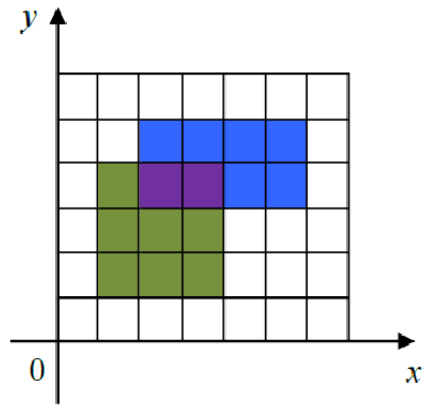
\includegraphics[scale=0.3]{paint}};

\node[anchor=north,text width=.2\textwidth] at(t1.south) {
	输入样例\\	
	2 \\
	1 1 4 4\\ 
	2 3 6 5 \\
	输出样例\\	
	15
};
\end{tikzpicture}
\end{frame}

\begin{frame}[shrink,fragile]{例7: 画图(结构体数组), 定义结构体}
\begin{columns}[T]
\column{0.6\textwidth}
\textbf{\textcolor{blue}{思路:}}
\begin{enumerate}
	\item 二维数组grid[N][N]表示网格, 最左下方单元是grid[0][0]元素。
	\item 定义矩形结构体, 各矩形组成结构体数组;
	\item 计算最大矩形, 其覆盖的单元格初始化为0; 
	\item 每个矩形覆盖的单元格标记为1, 
	\item 最大矩形被标记的单元格即是被涂色的单位面积。
\end{enumerate}
\column{0.4\textwidth}
\begin{lstlisting}
#define N 100
//定义矩形结构体 
struct Rec
{
   int leftBottomX;
   int leftBottomY;
   int rightTopX;
   int rightTopY;
};
\end{lstlisting}
\end{columns}
\end{frame}

\begin{frame}[shrink,fragile]{例7: 画图(结构体数组), 输入输出}
\vspace{-0.3cm}
\begin{lstlisting}
void input(struct Rec *recs, int n) // 输入n个矩形
{
  int i;
  for(i=0;i<n;i++) 
     scanf("%d%d%d%d",&recs[i].leftBottomX, &recs[i].leftBottomY,
     	&recs[i].rightTopX,&recs[i].rightTopY);
}
void print(struct Rec *recs, int n) // 输出n个矩形
{
  int i;
  for(i=0;i<n;i++) 
    printf("%d,%d,%d,%d\n",recs[i].leftBottomX,recs[i].leftBottomY,
    	recs[i].rightTopX,recs[i].rightTopY);
} 
\end{lstlisting}
\medskip
\end{frame}

\begin{frame}[shrink,fragile]{例7: 画图(结构体数组),计算最大矩形}
\vspace{-0.3cm}
\begin{lstlisting}
struct Rec Largest(struct Rec res[], int n)//res表示n个矩形, 返回最大矩形
{
   struct Rec largest=res[0]; //假设第一个是最大矩形 
   int i;
   for(i=1;i<n;i++)
   {
      if(res[i].leftBottomX < largest.leftBottomX)
          largest.leftBottomX=res[i].leftBottomX;
      if(res[i].leftBottomY < largest.leftBottomY)
          largest.leftBottomY=res[i].leftBottomY;
      if(res[i].rightTopX > largest.rightTopX) 
          largest.rightTopX=res[i].rightTopX;
      if(res[i].rightTopY > largest.rightTopY) 
          largest.rightTopY=res[i].rightTopY;
   }
   return largest; 
} 
\end{lstlisting}
\end{frame}

\begin{frame}[shrink,fragile]{例7: 画图(结构体数组), 网格\lstinline$grid[N][N]$初始化与标记}
\vspace{-0.3cm}
\begin{lstlisting}
void grid1(struct Rec rec, int grid[][N])// rec区域, grid数组元素置1(标记) 
{
   int i,j;
   for(i=rec.leftBottomY;i<rec.rightTopY;i++)
       for(j=rec.leftBottomX;j<rec.rightTopX;j++)
           grid[i][j]=1;
}
void grid0(struct Rec largest, int grid[][N])//largest区域, grid数组置0 
{
   int i,j;
   for(i=largest.leftBottomY;i<largest.rightTopY;i++)
      for(j=largest.leftBottomX;j<largest.rightTopX;j++)
           grid[i][j]=0;
}
\end{lstlisting}
\end{frame}

\begin{frame}[shrink,fragile]{例7: 画图(结构体数组), 计算被标记的网格}
\begin{lstlisting}
// largest区域, 返回grid数组元素为1的单元数量,即被覆盖的单位面积数 
int gridNum(struct Rec largest, int grid[][N])
{
   int i,j,num=0;
   for(i=largest.leftBottomY;i<largest.rightTopY;i++)
   {
       for(j=largest.leftBottomX;j<largest.rightTopX;j++)
          if(grid[i][j]) num++;
   } 
   return num;
}
\end{lstlisting}
\end{frame}

\begin{frame}[shrink,fragile]{例7: 画图(结构体数组),主函数}
\vspace{-0.4cm}
\begin{lstlisting}
int main() // 模块化程序设计,便于调试。
{
    int grid[N][N],n,i,num;
    struct Rec recs[N],largest;
    scanf("%d",&n);
    input(recs,n);
    // print(recs,n); // 检查输入 
    largest=Largest(recs,n); // 计算最大矩形 
    // print(&largest,1); // 查看最大矩形是否正确 
    grid0(largest,grid); // 初始化 
    for(i=0;i<n;i++)
       grid1(recs[i],grid); // 标记网格, 置1 
    printf("%d\n",gridNum(largest,grid)); // 统计输出 
    return 0;
}
\end{lstlisting}
\end{frame}

\begin{frame}[shrink,fragile]{例8: 世界杯排名}
\begin{tikzpicture}
\node[text width=0.82\textwidth] (t) {
给出世界杯一个小组的小组赛成绩,请找出最终进入淘汰赛的球队。 \\
小组赛积分规则:胜一场积3分、平一场积1分、负一场积0分。 \\
小组赛排名规则如下: \\
1.首先按照积分排名,积分越高,排名越高\\ 
2.积分相同的队按照净胜球(进球数减去失球数)排名,净胜球越多,排名越高\\ 
\textcolor{blue}{输入说明:} 输入数据第一行为两个整数$N$和$M,N$表示小组中队伍数量$(N\le 32)$,$M$表示出线名额$(M\le 16)$。
接下来是$N$行数据,每一行表示一只队伍的小组赛比赛信息,
依次为队名(长度不超过20的字符串)、胜场数、平局数、负场数、进球数、失球数。
输入数据保证没有两个球队的积分和净胜球完全相同。

\textcolor{blue}{输出说明:} 根据题目给出的积分排名规则,按照排名从高到低顺序依次输出出线球队的排名(从1开始排名)、队名、积分和净胜球,
各个字段之间用空格分隔。
};
\node[anchor=west,text width=0.3\textwidth,draw] at($(t.east)+(0.5,0)$) {
	输入样例\\	
	4 2\\ 
	Germany 2	1	0	7	2 \\
	Portuguesa 1	1	1	4	7 \\
	America 1	1	1	4	4 \\
	Ghana 0	1	2	4	6 
	
	输出样例\\	
	1 Germany	7 5 \\
	2 America 4 0 
};
\end{tikzpicture}
\end{frame}

\begin{frame}[shrink,fragile]{例8: 世界杯排名, 定义结构体}
\begin{columns}[T]
\column{0.4\textwidth}
\textbf{\textcolor{blue}{思路:}}
\begin{enumerate}
	\item 定义结构体存储球队相关信息;
	\item 各球队组成结构体数组;
	\item 按要求对结构体数组进行排序。
\end{enumerate}
\begin{lstlisting}
// 估计最大数 
#define N 32
#define M 16
\end{lstlisting}
\column{0.5\textwidth}
\begin{lstlisting}
// 定义结构体类型,存储球队相关信息 
struct Team
{
  char name[20];
  int win,draw,lose; // 胜,平,负场数 
  // 进球数,失球数
  int goalsNum,losesNum; 
  int grades; // 积分
  int goals;  // 净胜球  
};
\end{lstlisting}
\end{columns}
\end{frame}

\begin{frame}[shrink,fragile]{例8: 世界杯排名, 输入}
\begin{lstlisting}
// 输入n个球队信息, 根据规则填充结构体成员
void input(struct Team *teams, int n)
{
   for(i = 0; i < n; i++)
   {
      scanf("%s%d%d%d%d%d",teams[i].name,&teams[i].win,&teams[i].draw,
      		&teams[i].lose,&teams[i].goalsNum,&teams[i].losesNum);
      // 根据规则填充其它数据成员
      teams[i].grades =  teams[i].win*3 + teams[i].draw*1;
      teams[i].goals = teams[i].goalsNum - teams[i].losesNum; 
   }
}
\end{lstlisting}
\end{frame}

\begin{frame}[shrink,fragile]{例8: 世界杯排名, 交换函数}
\begin{columns}[T]
\column{0.8\textwidth}
\begin{lstlisting}
// 交换两个结构体指针的内容, 地址传递
// 两个结构体的各数据成员互相交换 
void swap(struct Team *team1, struct Team *team2)
{
   struct Team tmp;
   tmp = *team1; 
   *team1 = *team2; 
   *team2 = tmp;
}
\end{lstlisting}
%\column{0.5\textwidth}
\end{columns}
\medskip
\end{frame}

\begin{frame}[shrink,fragile]{例8: 世界杯排名, 排序}
\vspace{-0.5cm}
\begin{columns}[T]
\column{1.5\textwidth}
\begin{lstlisting}
void sorts(struct Team a[], int n)// 定义排序函数(选择法,降序): 按积分和净胜球排序 
{
   int i,j,k;
   for(i = 0; i < n - 1; i++)
   {
      k = i; // 未经排序较大者
      for (j = i+1; j < n; j++)
      {
         // 条件判断语句:善用&&、||运算,简化if else结构 
        if (a[j].grades > a[k].grades || 
           (a[j].grades == a[k].grades &&  a[j].goals > a[k].goals))  
              k = j;
      }
      if (k != i) swap(&a[i],&a[k]); // 交换
   } 
}
\end{lstlisting}
\end{columns}
\medskip
\end{frame}

\begin{frame}[shrink,fragile]{例8: 世界杯排名,主函数}
\vspace{-0.4cm}
\begin{lstlisting}
// 模块化程序设计,便于调试。
int main()
{
   struct Team teams[N]; // 以估计最大数,定义结构体数组 
   int n,m,i;
   scanf("%d%d",&n,&m);
   input(teams,n); 
   sorts(stus,n); // 排序
   // 输出前m个排序后的球队 
   for(i = 0; i < m; i++)
      printf("%d %s %d %d\n",i+1,teams[i].name,teams[i].grades,
      		teams[i].goals);
   return 0;
}
\end{lstlisting}
\end{frame}

\begin{frame}{复习指引}
\vspace{-0.2cm}
\begin{columns}
	\column{0.7\linewidth}
	\begin{itemize}
		\item 认真复习ppt及百道练习题,确保不犯低级错误。
		\item 认真复习ppt及百道练习题,深刻体会编程思路。
		\item 认真复习ppt及百道练习题,注重一题多解,总结自己的编程宝典,做到遇类似问题,脑洞大开。
		\item 善用标志变量(如, 跳一跳, 字符计数,连续1等练习题),标志矩阵(如, 消费类游戏, 购票系统等练习题)。
		\item 善用函数,简化程序设计。
		\item 应用结构体和函数得到逻辑简单, 思路清晰的程序。貌似复杂的问题迎刃而解。 
	\end{itemize}
	\column{0.3\linewidth}
	\centering
\includegraphics[scale=0.2]{timg}
\end{columns}
\end{frame}

